\chapter{Tecnica Ottimizzata}
\label{cap:3}
In questo capitolo viene presentata un'ottimizzazione al problema descritto nel capitolo precedente.
Tale ottimizzazione si basa sul principio delle decomposizioni bilanciate.
Si fa vedere, inoltre, come l'utilizzo di quest'ultima permetta un notevole miglioramento delle performance.

\section{Decomposizioni Bilanciate di un albero}
\label{cap:3 par:1}
Si vuole andare a dimostrare in questa sezione che dato un albero T \`e sempre possibile ricavare una scomposizione bilanciata dell'albero.
\\
Prima di poter enunciare e dimostrare il risultato principale occorre dare delle nozioni preliminari.

\newtheorem{definizione}{Definizione}[section]

\begin{definizione}
	\label{definizioneDeco}
Sia $T_r$ un albero radicato nel nodo r, con k nodi.
Diremo che la coppia (A,B), dove  A e B sono insiemi contenenti i nodi di $T_r$, \`e una decomposizione per l'albero $ T_r $ se:
\begin{itemize}
	\item $| A | + | B | = k$
	\item $A \cap B = \{r\}$.
\end{itemize}
\end{definizione}


\begin{definizione}
\label{lemmaDeco}
Dato un albero $ T $ con $ k $ nodi, diremo che $ (A,B) $ \`e una decomposizione bilanciata se:
\begin{equation*}
	\max{ \{|A| , |B| \} }  \le  f(k)
\end{equation*}
dove $ f $ \`e una funzione definita su $ k $.
\end{definizione}





\begin{definizione}
Per ogni nodo $ v $ di un albero $ T $, le diramazioni di $ T $  rispetto a $ v $, sono tutti i sottoalberi massimali di $ T $ non contenenti $ v $. 
Per ogni $ v \in T $, si definisce $\alpha(v)$ come il grado della diramazione di $ v $ con il maggior numero di nodi.\\
Un nodo $ v $ di un albero $ T $ con $ n $ nodi, \`e un nodo centroide se $\alpha(v)\le\frac{n}{2}$.
\end{definizione}\mbox{}

Il centroide di un albero non \`e necessariamente unico, infatti Jordan \cite{jordan1869assemblages}  ha dimostrato che, dato un albero $ T $ con $ n $ nodi:
\begin{enumerate}
	\renewcommand{\labelenumi}{\roman{enumi}}
	\item $ T $ ha un singolo centroide $ v $ e $\alpha(v) < \frac{n}{2}$;
	\item$ T $ ha due nodi centroidi (adiacenti) $v_1$ e $v_2$ tali che $\alpha(v_1) = \alpha(v_2) = \frac{n}{2}$, in questo caso il numero di nodi $ n $ \`e pari.
\end{enumerate}

Esistono diversi algoritmi per la ricerca del centroide, quello utilizzato in questa tesi \`e l'algoritmo di Jordan \cite{jordan1869assemblages} che  ha una complessit\`a temporale lineare nel numero di nodi. \\
Il primo passo da effettuare \`e determinare $\alpha(v)$ per ogni nodo $ v \in T$.\\
Si definisce  $\delta(z)$ come il fattore di diramazione di un albero. ossia il numero di nodi incontrati durante una visita DFS (in profondit\`a) effettuata a partire dalla radice $ z $.
Siano $\delta(z_i)$ i fattori di bilanciamento ottenuti da tutte le possibili diramazioni $ i $ di $ T $ unite a $ v $, che non lo contengono, allora, $ \alpha(v) = \max \{\delta(z_i)\} $.

Una volta calcolato il valore di $ \alpha(v) $ $ \forall v \in T $ si verifica per quali valori  risulta $\alpha(v)\le\frac{n}{2}$.
Nel caso ci fosse un unico nodo $ v $ che soddisfa la precedente espressione,, come in (i),  allora tale nodo rappresenta l'unico  centroide dell'albero $ T $.
Nel caso, invece, ce ne fossero due, come definito in (ii), per esempio $ v_1 $ e $ v_2 $,  l'albero $ T $ conterr\`a due centroidi, rispettivamente $ v_1 $ e $ v_2 $.\\
Nell'esempio \ref{es1} si pu\`o vedere l'applicazione dell'algoritmo per la ricerca del centroide.
	\begin{figure}[htbp]
		\centering
		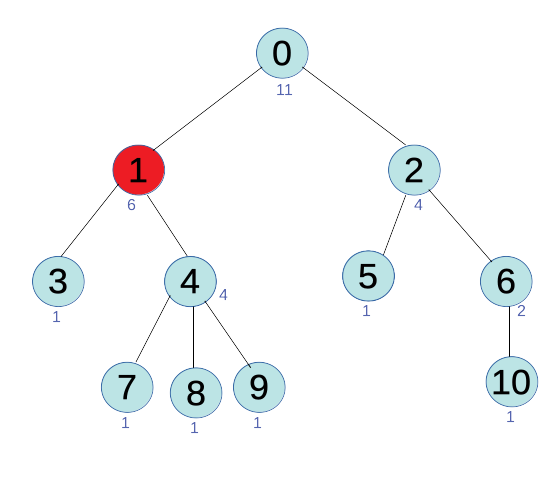
\includegraphics[width=5cm]{capitolo3/grafo2}
		\caption{Albero $ T $  per la ricerca del centroide} 
		\label{fig:2}
\end{figure}
\mbox{}\\

\newtheorem{esempio}[definizione]{Esempio}
\begin{esempio}
	\label{es1}
Si consideri l'albero T in figura \ref{fig:2} per la ricerca del nodo centroide.
Per ogni nodo $ v $ di $ T $, numerato da 0 a 10,  viene calcolato $\alpha(v)$ . \\
Quello che si ottiene \`e :


\begin{center}
	\begin{tabular}{ c c c c c  }
		$\alpha(0) = 6$ & & $\alpha(1) = 7$ & & $\alpha(2) = 5$ \\ 
		$\alpha(3) = 9$ && $\alpha(4) = 10$ &&  $\alpha(5) =  7$ \\  
		$\alpha(6) = 10$ && $\alpha(7) = 10$ && $\alpha(8) = 10$ \\
		$\alpha(9) = 10$ && $\alpha(10) = 10$ &&
	\end{tabular}
\end{center}

Poich\'e $ \left\lfloor\frac{n}{2} \right\rfloor = \left\lfloor \frac{11}{2} \right\rfloor = 5$, l'unico nodo per cui la disuguaglianza risulta vera \`e il nodo 2, infatti $5\le 5$, ed \`e esattamente l'unico centroide dell'albero T (figura \ref{fig:2}). 
\demo
\end{esempio}\mbox{}\\

L'ultimo punto da considerare prima di poter enunciare e dimostrare il risultato principale di questa sezione riguarda la definizione di un algoritmo valido per comporre due insiemi di nodi, che chiameremo $ T' $ e $ T'' $, in maniera $ f(k) $-bilanciata.\\
Siano dati in input un albero $ T $, con $ k $ nodi, ed un fattore di bilanciamento definito da una funzione $ f(k) $, poich\'e non considero la radice di $ T $, la funzione viene valutata su $ k-1 $ piuttosto che su $ k $.
Si suppone inoltre, senza perdita di generalit\`a, che i sottoalberi radicati nei figli della radice $ r $ di $ T $ siano ordinati con ordine non crescente.
Da questo deriva che, supponendo che $ r $ abbia $ n $ figli, vi saranno al pi\`u $  n $ alberi radicati in ciascuno di essi tali che: $ |T_i| \ge |T_{i+1}|$ \ $ \forall i = 1,\dots, n-1 $.\mbox{}\\\\

	\begin{figure}[htbp]
	\centering
	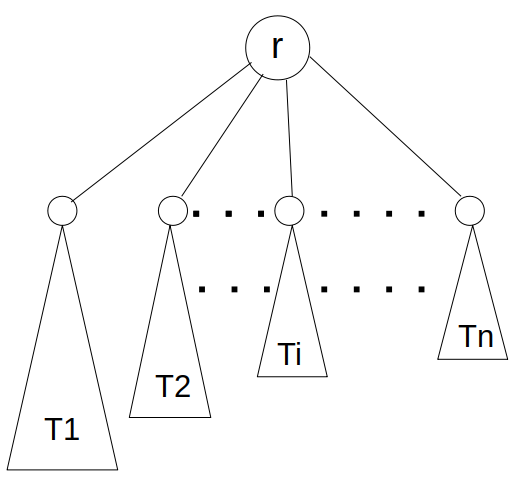
\includegraphics[width=5cm]{capitolo3/grafo3}
	\caption{Esempio di albero $ T $ radicato in $ r $, con $ k $ nodi, valido come input per l'algoritmo \ref{algoritmo1}} 
	\label{fig:3}
\end{figure}
\mbox{}\\

\begin{algorithm}[H]
	\label{algoritmo1}
	\SetAlgoLined
	\caption{Insiemi $ k $-bilanciati}
	\textbf{input} : Albero $ T $ con $ k $ nodi, fattore di bilanciamento $ f(k-1) $;\\
	$ |T'| , |T''|\longleftarrow $ due insiemi di nodi inizialmente vuoti;\\ 	
	\For{$ i = 1,\dots,n $}
	{
		\If{$ \sum_{j=1}^{i}{|T_j|} > f(k-1) $}
		{
			$ T'\longleftarrow $ sottoalbero di  di $ T $ indotto da $ \{r\} \cup \bigcup_{j=1}^{i-1}V(T_j)$.\\
			$ T''\longleftarrow $ sottoalbero di $ T $ indotto da $ V(T) \diagdown T'$.
		}
		 
}
	Restituisci ($ T',T'' $).

\end{algorithm}\mbox{}\\

Una volta concluso l'algoritmo \ref{algoritmo1} si avr\`a una coppia $ (T',T'') $ tale che : $ \max (|T'|,|T''|) \le f(k-1) $.
Viene pertanto rispettata la definizione \ref{lemmaDeco}, perci\`o si ottiene una decomposizione $ f(k-1) $-bilanciata.

In base a tutte le nozioni fino ad ora discusse si pu\`o dare il seguente risultato\mbox{}\\
.


\newtheorem{teorema1}[definizione]{Teorema}
\begin{teorema1}
	\label{teorema1 cap3 sez1}
Per ogni albero T di k nodi esiste un nodo r di T  tale che l'albero $T_r$, ottenuto radicando T in r, ammette una decomposizione $ (\lfloor \frac{2}{3}(k-1) \rfloor + 1)$-bilanciata ed, inoltre, sia $ (|T'|,|T''|)$ tale decomposizione risulta che il $ \max \{|T'|,|T''|\} \ge 2+ \left\lfloor \frac{(k-1)}{3}\right\rfloor $
\end{teorema1}\mbox{}
\begin{proof}
	
	Sia $ T $ un albero di $ k $ nodi,con $ k>2 $ (per $n\le2$ la propriet\`a \`e banalmente vera) \\
	La prima operazione da compiere \`e individuare il nodo $ r $ di $ T $ su cui si andr\`a poi a radicare il nuovo albero $ T_r $.\\
	Si suppone che tale nodo sia un centroide dell'albero $ T $ quindi si applica l'algoritmo di Jordan per la ricerca del centroide, senza perdita di generalit\`a si suppone di avere un unico nodo centroide, indicato con $ r $.\\
	Se il centroide $ r $ trovato non corrisponde alla radice dell'albero $ T $, si modifica $ T $ radicandolo in $ r $ e l'albero cos\`i ottenuto verr\`a indicato con $ T_r $. \\ 
	Inoltre, si suppone che i sottoalberi radicati nei figli di r siano ordinati in maniera non crescente rispetto alla loro dimensione.\\
	Si applichi a $ T_r $ l'algoritmo \ref{algoritmo1} precedentemente descritto per definire se \`e possibile ottenere una $ f(k) $-decomposizione, con $ f(k) =
	(\lfloor \frac{2}{3}(k-1) \rfloor + 1  $.\\
	Sia $ \{T_i \ | \  i=1,\dots,n\} $ l'insieme dei sottoalberi radicati negli $ n $ figli di $ r $ e si consideri il primo valore di $ i $ tale che l'istruzione $ if $ di riga $ 4 $ nell'algoritmo \ref{algoritmo1} risulti vera (si noti che tale valore di $ i $ esiste sempre dal fatto che per $ i = n $ la condizione \`e verificata).\mbox{}\\\\
	Sia 
	\[ S = \sum_{i=1}^{n}{|T_i|} = (k-1 ) \]\\
	e sia
	\[ x = \sum_{j=1}^{i-1}{|T_j|} \]\\
	Distinguiamo due casi
	\begin{itemize}
	\item $\textbf{ i>2 }$ Si ha che
	\\ 
	\begin{equation}\label{1}
		x+|T_i| > \frac{2}{3}\cdot S
	\end{equation}
\\
	Inoltre sapendo che
	\\
	
	\begin{equation}\label{2}
	|T_i| \le \frac{S}{i} \le \frac{S}{3}	
	\end{equation}
\\
		
	Sottraendo la disequazione \eqref{2} alla \eqref{1} si ottiene che 
	\\
	\begin{equation}\label{3}
	x > \frac{2}{3}\cdot S - \frac{S}{3} = \frac{S}{3}	
	\end{equation}
\\
 	\item $ \textbf{i=2} $ Anche in questo caso come nel precedente vale la disequazione \eqref{1}.\\
 	Inoltre, essendo $ i = 2 $ per costruzione dell'albero $ T $ si pu\`o dire che
 	
 	\begin{equation}\label{4}
 	x = |T_1| \ge |T_2| = |T_i|
 	\end{equation}
 	
 	Pertanto, sfruttando la disequazione \eqref{4} combinata con la \eqref{1} si ha che
 	\begin{equation}\label{5}
 	2x > \frac{2}{3} \cdot S \Rightarrow x > \frac{S}{3}
 	\end{equation}
	\end{itemize}\mbox{}\\


Per entrambi i casi otteniamo che 
\\
\[ x > \frac{S}{3} \Rightarrow x \ge \left\lfloor \frac{S}{3}\right\rfloor  + 1 \]
\\

Pertanto si avr\`a che 
\\
\[ \left\lfloor \frac{S}{3}\right\rfloor  + 1 \le x \le \left\lfloor \frac{2}{3}\cdot S \right\rfloor \] 
\\

Quindi 
\\
\begin{equation}\label{5}
|T'| = 1+x \le 1 + \left\lfloor \frac{2}{3}\cdot S \right\rfloor = 1 + \left\lfloor \frac{2}{3} \cdot (k-1) \right\rfloor	
\end{equation}
\\
\begin{equation}\label{6}
|T''| = 1 + S - x = 1+S-1 - \left\lfloor \frac{S}{3}\right\rfloor = \left\lceil \frac{2}{3}\cdot S \right\rceil = \left\lceil \frac{2}{3} \cdot (k-1) \right\rceil 	
\end{equation}
\\
Inoltre
\\
\[ |T'| = 1+ x \ge 1+ (1 +  \left\lfloor \frac{S}{3}\right\rfloor ) = 2 +  \left\lfloor \frac{(k-1)}{3}\right\rfloor\]
\\
Poich\`e
\\
 	 \[1 + \left\lfloor \frac{2}{3} \cdot (k-1) \right\rfloor \ge \left\lceil \frac{2}{3} \cdot (k-1) \right\rceil \]
 	 \\

Possiamo concludere che
\\

\[2 +  \left\lfloor \frac{(k-1)}{3}\right\rfloor \le \max\{|T'|,|T''|\} \le 1 + \left\lfloor \frac{2}{3} \cdot (k-1) \right\rfloor \]
 \\
ottenendo perci\'o una decomposizione $ (\lfloor \frac{2}{3}(k-1) \rfloor +1)$-bilanciata, tale che $ \max \{|T'|,|T''|\} \ge 2+ \left\lfloor \frac{(k-1)}{3}\right\rfloor $	 
 	 
\end{proof}\mbox{}\\
 
 	Nel caso in cui si abbiano due centroidi, la scelta su quale radicare l'albero  \`e deterministica.\\
 	Nel caso in cui gli alberi ottenuti radicando $ T $ in ognuno di essi abbiano strutture differenti, viene scelto quello che tra i due ha una struttura pi\`u piccola.
 	Altrimenti se gli alberi ottenuti sono identici, viene scelto uno dei due in maniera arbitraria.
 	
\section{Algoritmo}
\label{cap:3 par:2}
In questa sezione si vede come \`e stato utilizzato il risultato del paragrafo \ref{cap:3 par:1} per ottimizzare e migliorare l'algoritmo \ref{algoritmo} descritto nel capitolo \ref{cap 2} paragrafo \ref{section1}.\\
Molto brevemente, quello che si faceva precedentemente era la seguente cosa.
Dato $ T_C = (T,C) $, con $ T $ un albero colorato radicato di $ k $ nodi i cui colori giacciono in $ C $, si procedeva a calcolare il numero di occorrenze $ c(T_C,v) $ \ $ \forall v \in V $ dividendo idealmente $ T $ in due sottoalberi $ T' $ e $ T'' $ con $ T'' $ il sottoalbero radicato in uno dei figli della radice di $ T $ e $ T'$ il sottoalbero di $ T $ , radicato in $ r $ contenente $ |T | - |T'' | $ nodi. 
Si procedeva al conteggio delle occorrenze di $ T_C $ nel seguente modo
\[	c(T_c,v)=\frac{1}{\beta_T}\sum_{(u,v)\in E}\sum_{\substack{C' \subset C \\C'' = C \setminus C' \\ |C'|=|T'|, |C''| = |T''|}}c(T'_{C'},v)\cdot c(T''_{C''},u)\]   

In questa nuova versione, invece, la divisione dell'albero $ T_C $ non \`e pi\`u scelta in maniera ideale, ma bens\`i vengono presi due alberi $ T'_{C'} $ e $ T''_{C''} $ tali che la decomposizione di $ T_C $ risulti bilanciata.
Inoltre, a differenza della precedente versione, gli alberi $ T'_{C'} $ e $ T''_{C''} $ saranno radicati entrambi nello stesso nodo $ v $ su cui sar\`a poi radicato $ T_C $.



